\chapter*{ПРИЛОЖЕНИЕ A}
\addcontentsline{toc}{chapter}{ПРИЛОЖЕНИЕ A}

%<слайды презентации>

\begin{figure}[ht!]\centering
	
\includegraphics[width=\linewidth]{pres_1}
	\caption{Титульный слайд (слайд 1)}
\end{figure}

\begin{figure}[ht!]\centering
	
\includegraphics[width=\linewidth]{pres_2}
	\caption{Цельи задачи работы (слайд 2)}
\end{figure}

\begin{figure}[ht!]\centering
	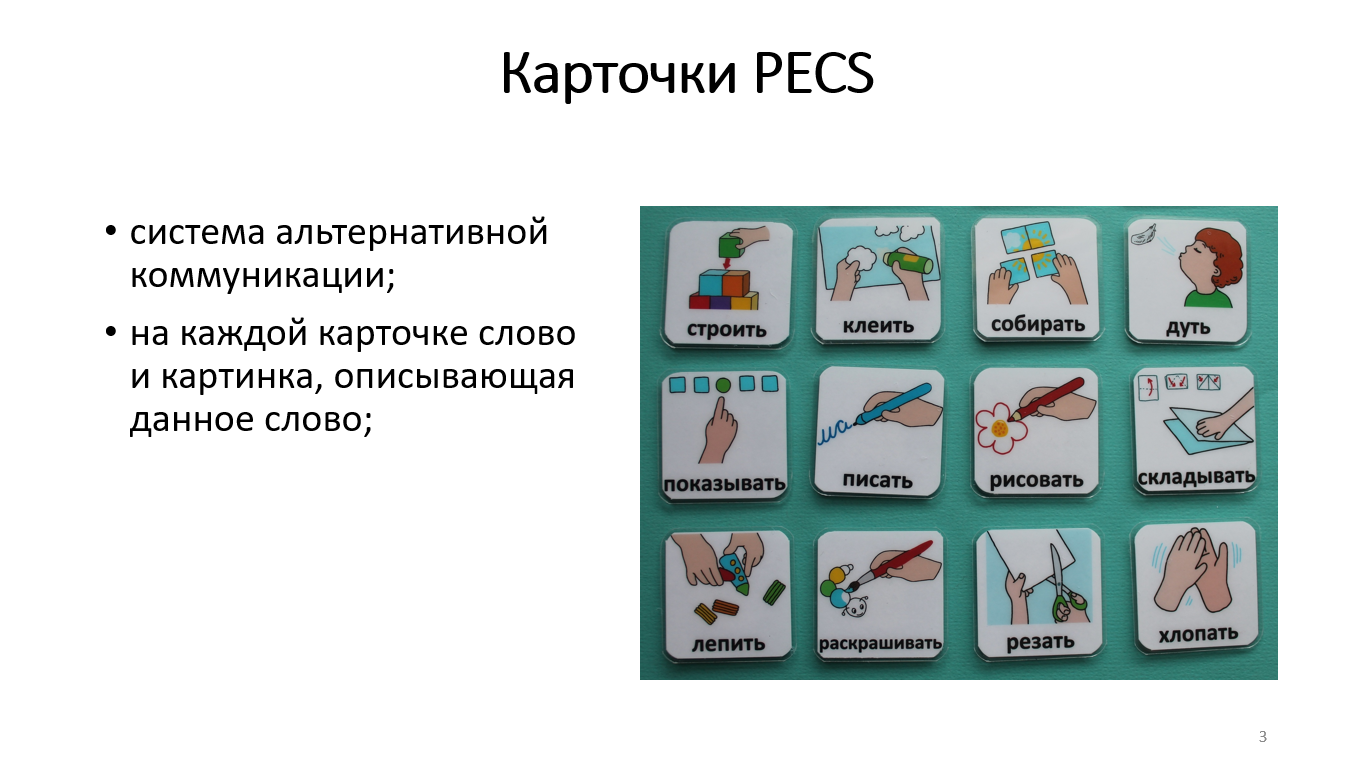
\includegraphics[width=\linewidth]{pres_3}
	\caption{Карточки PECS (слайд 3)}
\end{figure}

\begin{figure}[ht!]\centering
	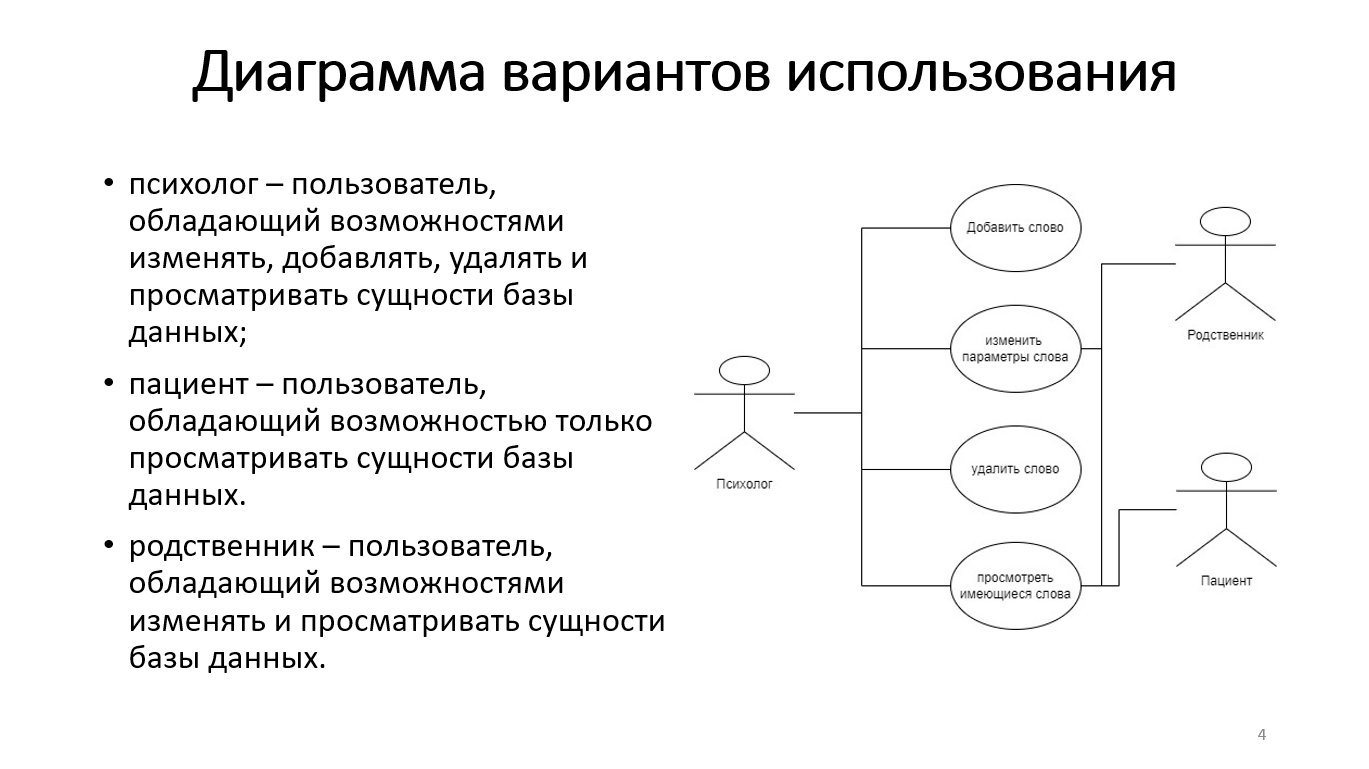
\includegraphics[width=\linewidth]{pres_4}
	\caption{Диаграмма вариантов использования (слайд 4)}
\end{figure}

\begin{figure}[ht!]\centering
	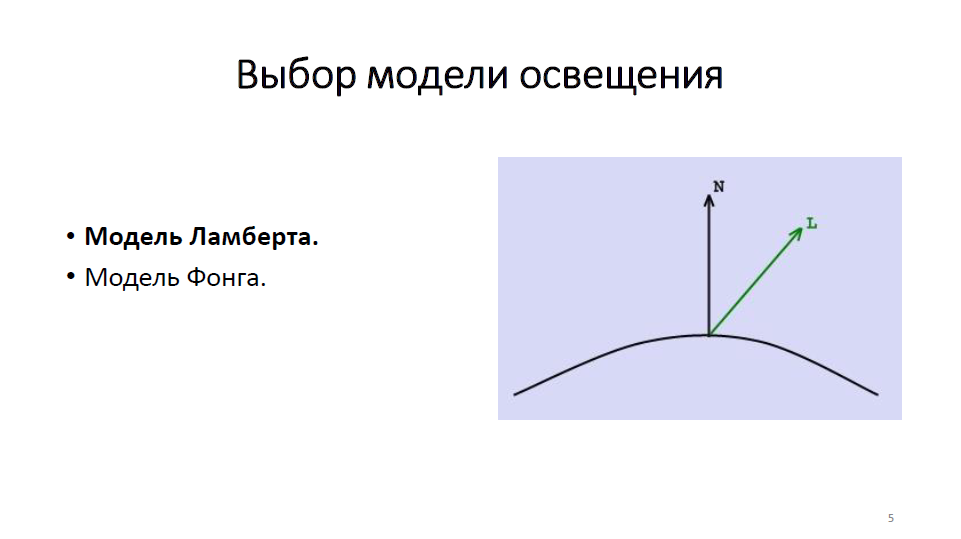
\includegraphics[width=\linewidth]{pres_5}
	\caption{ER-диаграмма в нотации Чена (слайд 5)}
\end{figure}

\begin{figure}[ht!]\centering
	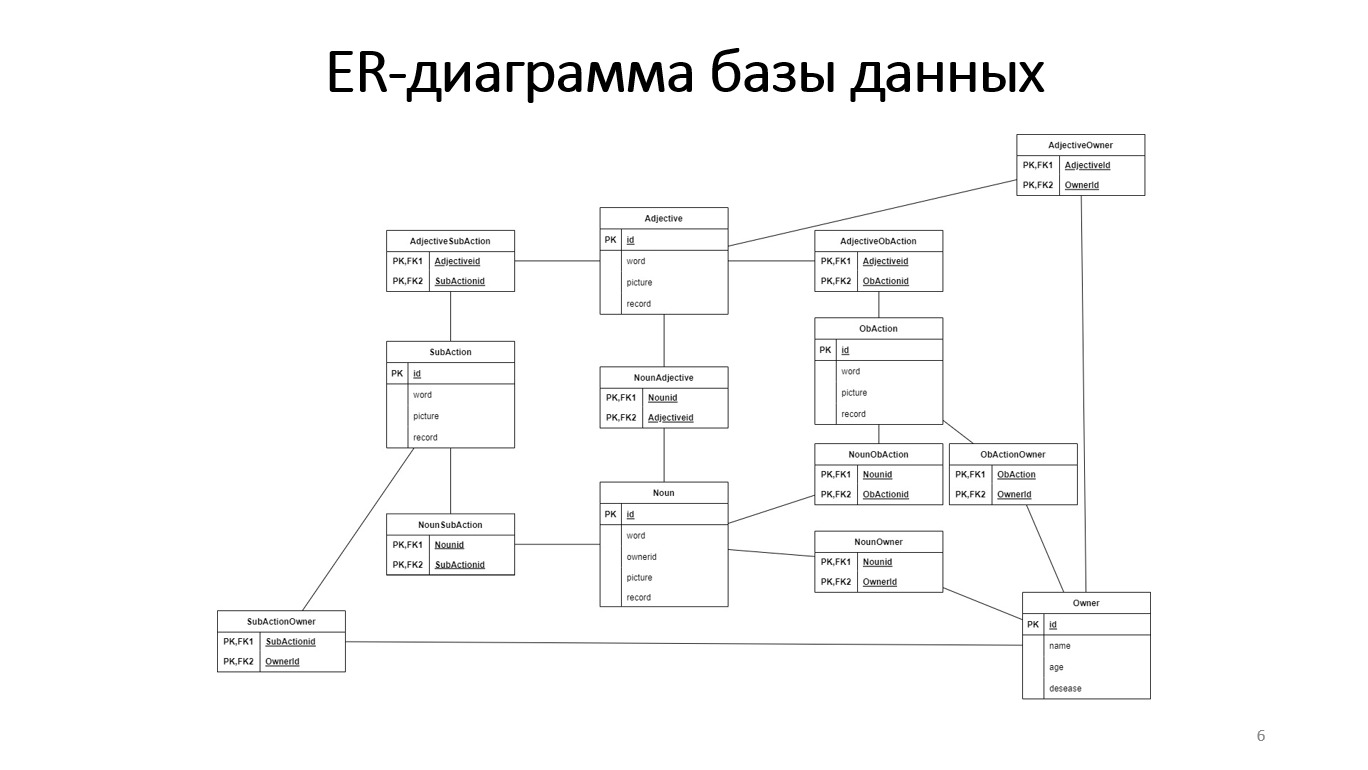
\includegraphics[width=\linewidth]{pres_6}
	\caption{ER-диаграмма базы данных (слайд 6)}
\end{figure}

\begin{figure}[ht!]\centering
	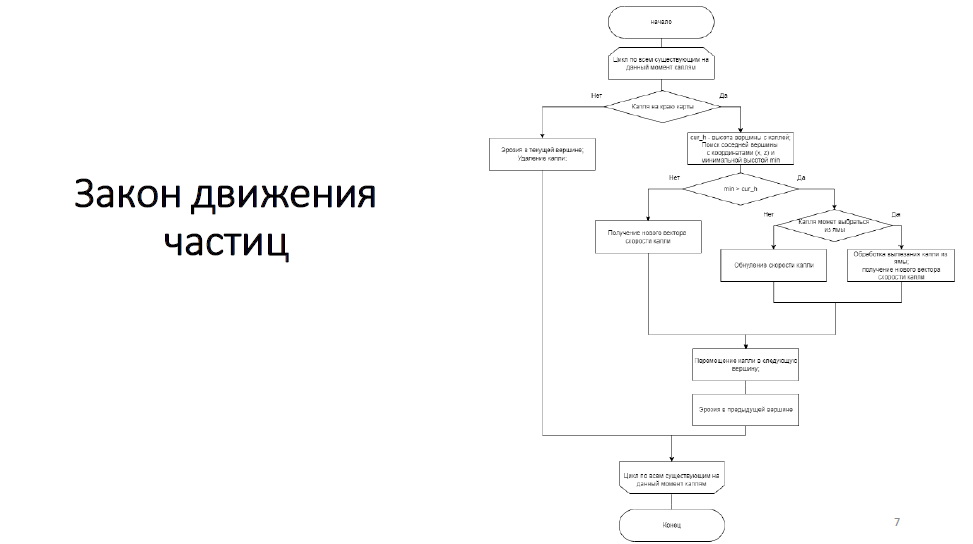
\includegraphics[width=\linewidth]{pres_7}
	\caption{Схема триггера (слайд 7)}
\end{figure}

\begin{figure}[ht!]\centering
	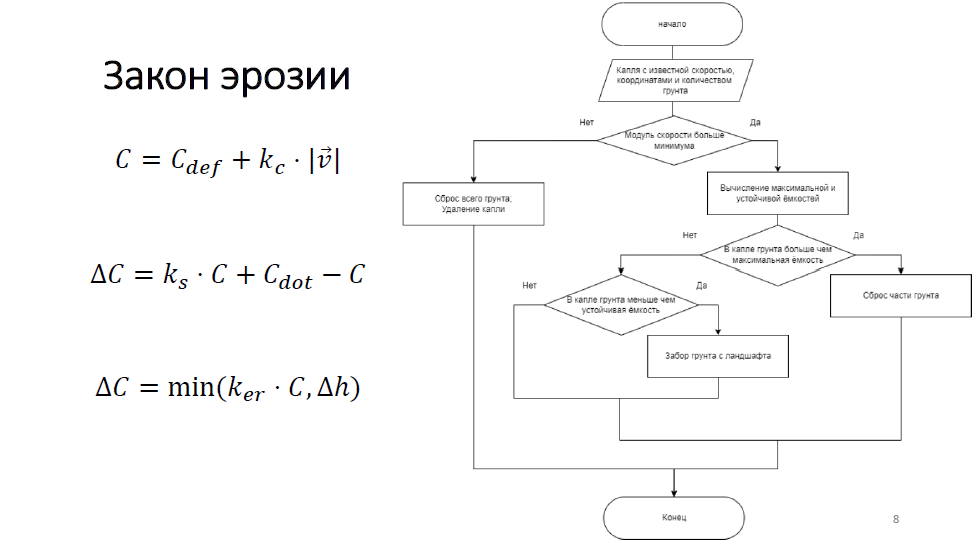
\includegraphics[width=\linewidth]{pres_8}
	\caption{Преимущества графвой БД (слайд 8)}
\end{figure}

\begin{figure}[ht!]\centering
	
\includegraphics[width=\linewidth]{pres_9}
	\caption{Выбранный технологический стек (слайд 9)}
\end{figure}

\begin{figure}[ht!]\centering
	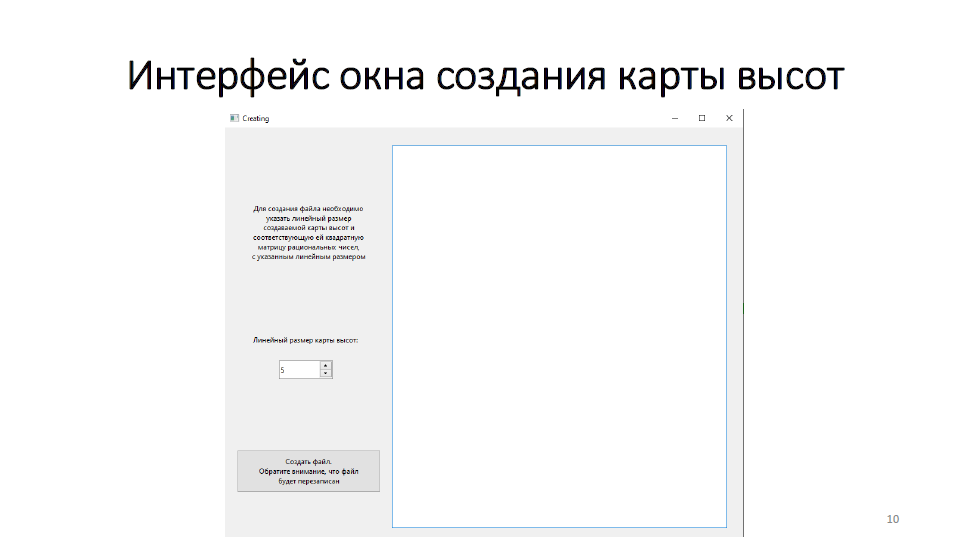
\includegraphics[width=\linewidth]{pres_10}
	\caption{Интерфейс взаимодействия (слайд 10)}
\end{figure}

\begin{figure}[ht!]\centering
	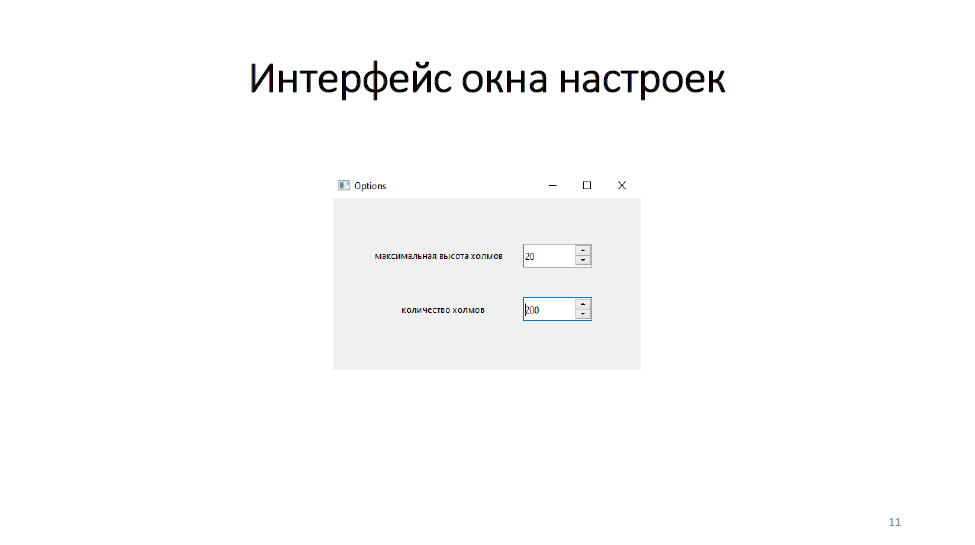
\includegraphics[width=\linewidth]{pres_11}
	\caption{Пример работы программы (слайд 11)}
\end{figure}

\begin{figure}[ht!]\centering
	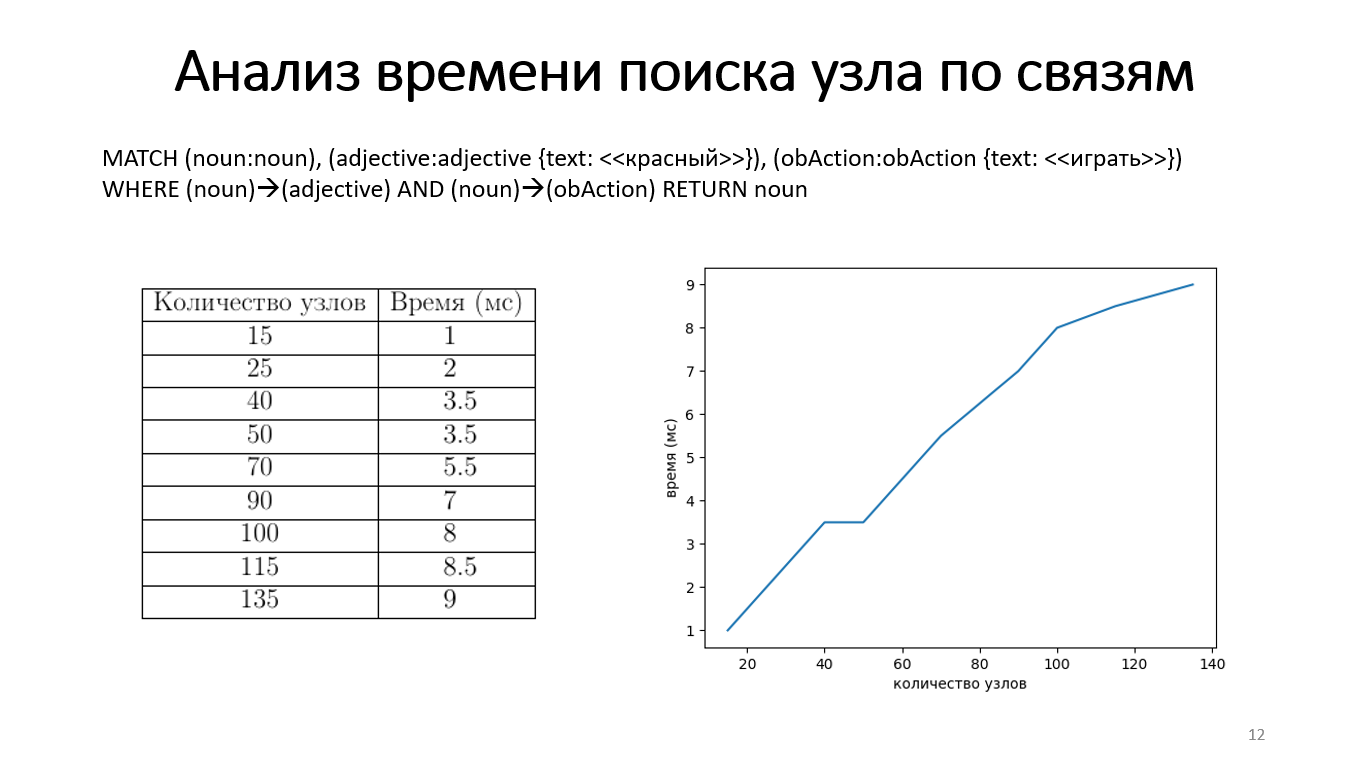
\includegraphics[width=\linewidth]{pres_12}
	\caption{Анализ времени поиска узла по связям (слайд 12)}
\end{figure}

\begin{figure}[ht!]\centering
	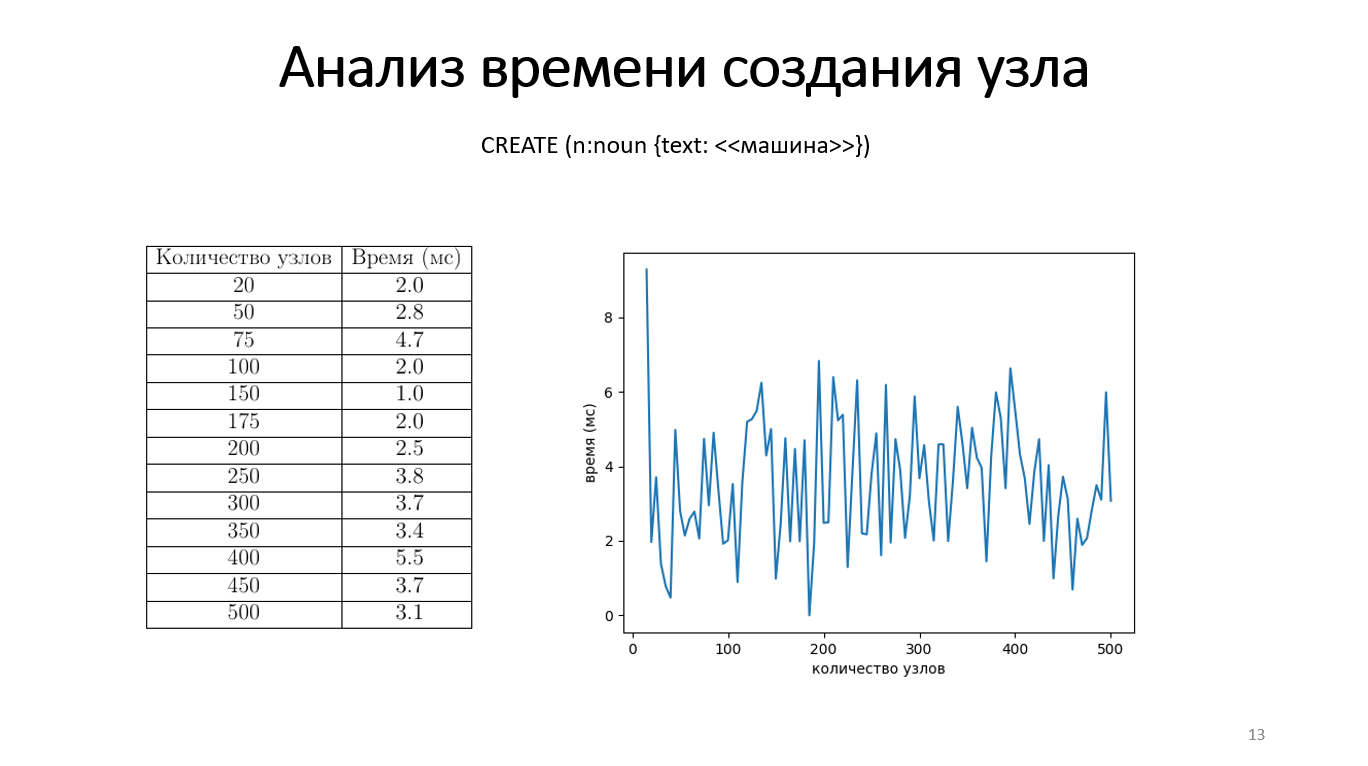
\includegraphics[width=\linewidth]{pres_13}
	\caption{Анализ времени создания узла (слайд 13)}
\end{figure}

\begin{figure}[ht!]\centering
	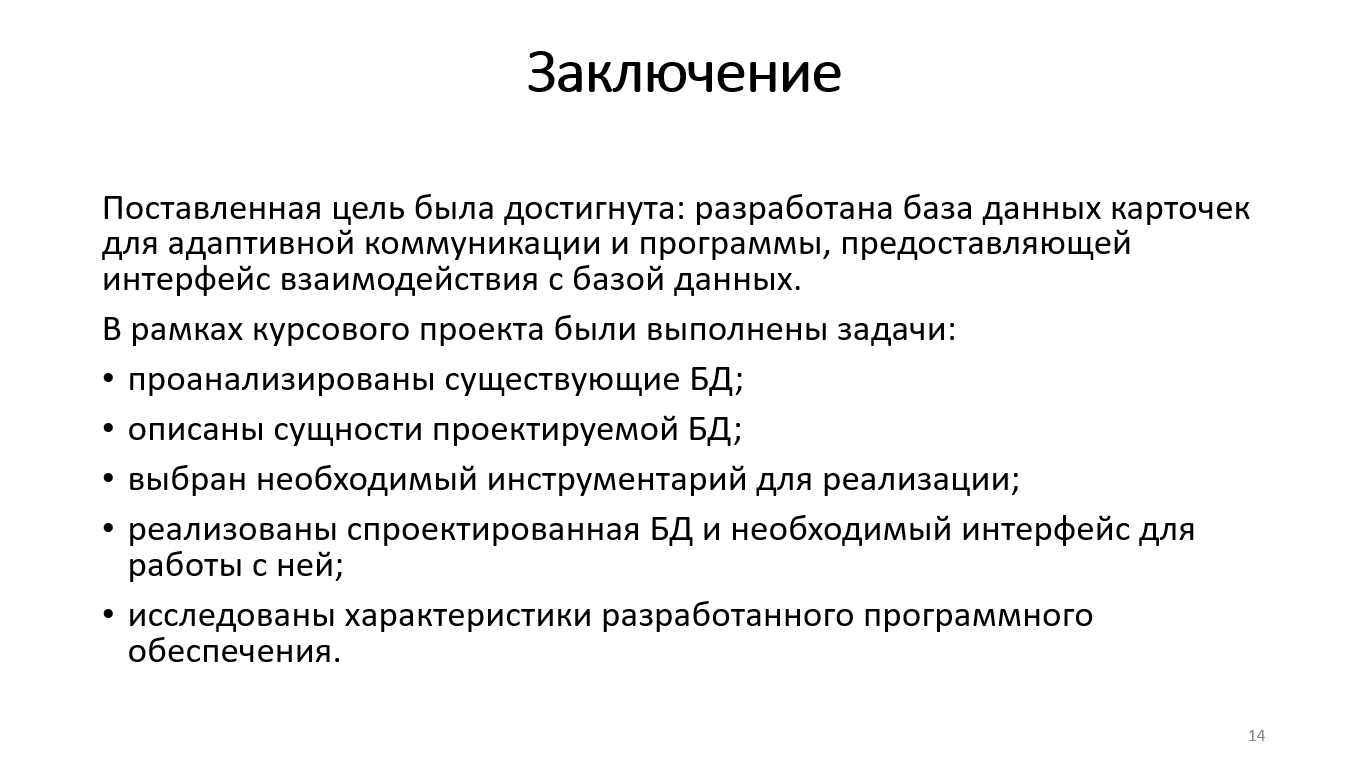
\includegraphics[width=\linewidth]{pres_14}
	\caption{Заключение (слайд 14)}
\end{figure}

\begin{figure}[ht!]\centering
	
\includegraphics[width=\linewidth]{pres_15}
	\caption{Направления дальнейшего развития (слайд 15)}
\end{figure}
